\subsection{Abstract Domains}\label{subsec:abstract-domains}

In the following section we will describe the abstract domains of our value analysis.

\subsubsection{Abstract strings as regular expressions}\label{subsubsec:abstract_domains_strings}
We have chosen regular expressions/languages to represent the abstract domain of the family of SQL string data types.
Regular expressions/languages are used instead of more powerful representations because of the decidable nature of inclusion and equality between them.

Let $\regexs$ denote the set of regular expressions; for elements of $\regex \in \regexs$, we denote the language of $\regex$ as $\lang(\regex)$.
In general, we will not distinguish between $R$ and $\lang(\regex)$ when it simplifies matters.
The lattice of $(\regexs, \subseteq, \cup, \cap)$ is a lattice but not a finite one; this is a problem: Essentially, we want the state-space of our analysis to be finite, such that we can employ the Kleene fixed-point theorem (see \autoref{thm:kleene_finite}) to prove the termination of our analysis.
If the state-space is built from infinite parts, the state-space itself will be infinite.
We will correct this problem later in \autoref{subsubsec:cover-lattice}.

\subsubsection{Abstract integers as union intervals}\label{subsubsec:abstract_domains_numbers}
We have chosen a finite union and intersection of intervals to represent the abstract domain of the family of SQL number data types.
Using a finite union ensures that operations such as union, intersection, and membership checking remain computable and efficient, which would not be feasible with infinite unions due to their inherent computational complexity.
We call them a union of intervals as all such objects can be written as a union of intervals.
We only consider integers, but the domain can be easily extended to the reals.
Let $\mathbf{INT}$ be the set of union intervals, with members denoted $\mathscr{I}$, that is inductively defined as:


\begin{gather*}
    \inference{i \text{ is an interval}}{i \in \mathbf{INT}} \quad
    \inference{\mathscr{I}_1 \in \textbf{INT} \quad \mathscr{I}_2 \in \textbf{INT}}{\mathscr{I}_1 \cup  \mathscr{I}_2 \in \mathbf{INT}}\\
    \inference{\mathscr{I}_1 \in \textbf{INT} \quad \mathscr{I}_2 \in \textbf{INT}}{\mathscr{I}_1 \cap  \mathscr{I}_2 \in \mathbf{INT}}
\end{gather*}


For the set of integers $\mathbb{Z}$, we will only consider $\emptyset, [a, b], [a, +\infty]$ and $[-\infty, b]$ where $a \leq b$ and $a, b \in \mathbb{Z}$, as valid intervals.

We define the language of union intervals as follows:


\begin{align*}
    \lang(\uint_1 \cup \uint_2) &= \lang(\uint_1) \cup \lang(\uint_2) \\
    \lang(\uint_1 \cap \uint_2) &= \lang(\uint_1) \cap \lang(\uint_2) \\
    \lang(\emptyset) &= \emptyset \\
    \lang([a, b]) &= \left\{ n \in \nums \middle| a \leq n \leq b \right\} \\
    \lang([a, +\infty]) &= \left\{ n \in \nums \middle| a \leq n \right\} \\
    \lang([-\infty, b]) &= \left\{ n \in \nums \middle| n \leq b \right\}
\end{align*}


As for the abstract domain of strings, we generally don't distinguish between a union interval $\uint$ and its language $\mathcal{L}(\uint)$ when it simplifies matters.
Furthermore, this abstract representation of numbers $(\uints, \subseteq, \cup, \cap)$ has the same issue as regular expressions: It is not finite.

This abstract domain is most likely not a new development, the title of~\cite{li2010abstract} suggest a similar construct, but we have been unable to get a hold of their paper.

\subsubsection{Cover lattices}\label{subsubsec:cover-lattice}
To resolve the issues presented above, we introduce the notion of a cover lattice.
As above the idea presented here is probably not novel.

Before we can define a cover lattice, we need to define the notion of a top-cover.

\begin{definition}
    A finite non-empty subset $X \subseteq S$ of a lattice $(S, \subseteq, \cup, \cap)$ is called a top-cover of $S$ whenever $\bigcup X = \top$.
\end{definition}

\begin{definition}\label{def:coverlattice}
Given a top-cover $X$ of a lattice $(S, \subseteq, \cup, \cap)$.
A cover lattice of $S$ in respect to $X$ denoted $\clattice{X}{S}$ is the set inductively defined as:

\begin{gather*}
    \inference{x \in X}{x \in C_X(S)} \quad
    \inference{x_1 \in C_X(S) \quad x_2 \in C_X(S)}{x_1 \cup  x_2 \in C_X(S)}\\
    \inference{x_1 \in C_X(S) \quad x_2 \in C_X(S)}{x_1 \cap  x_2 \in C_X(S)}
\end{gather*}
\end{definition}

As a note when we use the notation $C_X(S)$ we always assume that $X$ is a top-cover of $S$.
The notion of a cover lattices gives rise to the following theorem:

\begin{restatable}{theorem}{partition}\label{thm:partition}
For a non-complete lattice $(S, \subseteq, \cup, \cap)$ and top-cover $X$ of $S$, the cover lattice $(\clattice{X}{S}, \subseteq, \cup, \cap)$ is a finite and complete lattice.
\end{restatable}

And the following corollary's immediately follow:

\begin{corollary}
    If $\mathcal{R}$ is a top-cover of $(\regexs, \subseteq, \cup, \cap)$ then $(\clattice{\mathcal{R}}{\regexs}, \subseteq, \cup, \cap)$ is a finite and complete lattice.
\end{corollary}

\begin{corollary}
    If $\mathcal{I}$ is a top-cover of $(\uints, \subseteq, \cup, \cap)$ then $(\clattice{\mathcal{I}}{\uints}, \subseteq, \cup, \cap)$ is a finite and complete lattice.
\end{corollary}

We now define the function that maps elements in a lattice to the most precise element in a corresponding cover lattice:

\begin{align}
    \cdot \into C_X(S) &: S\rightarrow C_X(S) \\
    s \into C_X(S) &= \bigcap\{s' \in C_X(S)|s \subseteq s'\}
\end{align}

We overload this notation to work on sets of values in particular for $S' \subseteq S$ we define:

\begin{align}
    \cdot \into C_X(S) &: \mathcal{P}(S) \rightarrow \mathcal{P}(C_X(S)) \\
    S' \into C_X (S) &= \{s \into C_X(S) \mid s \in S'\}
\end{align}

To make this notion useful we assume that some mapping from application variables and table attributes to cover lattices is given by the user by some mechanism:

\begin{equation}\label{eq:lookupcl}
    \lookupcl : \mathbb{V}_t \cup \mathbb{V}_a \rightarrow \{ C_{X_1}(S_1), C_{X_2}(S_2), \dots, C_{X_n}(S_n) \}
\end{equation}


Where for all $1 \leq i \leq n$ either $S_i = \regexs$ with some $X_i = \mathcal{R} \subset \regexs$ or $S_i = \uints$ with some $X_i = \mathcal{I} \subset \uints$.
Further we define the following helper function:


\begin{align}
    c(C_{\mathcal{R}}(\regexs)) &= \strs \\
    c(C_{\mathcal{I}}(\uints)) &= \nums
\end{align}


Where $\strs$ are the set of all strings and $\nums$ the set of all integers.

Now we are able to express the concretization for regular expressions and union intervals.

\begin{align}
    &\concrete^v_6 : \lookupcl(v) \rightarrow \cc(\lookupcl(v)) \\
    &\concrete^v_6(X) = \mathcal{L}(X)
\end{align}

% \begin{definition}
%     We define $\cdot \into C_X(S):S\rightarrow C_X(S)$ to be the function mapping $s\in S$ to the least element in $C_X(S)$ containing it, that is $s \into C_X(S)=\bigsqcap\{s'\in C_X(S)|s\sqsubseteq s'\}$
%     \\
%
%     We define $\cdot \into C_X(S):\mathcal{P}(S)\rightarrow \mathcal{P}(C_X(S))$ to be the function that maps the powerset$(\mathcal{P})$ of the lattice elements to the powerset of the cover lattice elements$(C_X (S))$.
%     We use $H \into C_X (S) = \{h \into C_X (S) \mid h \in H\}$ to show how a set of elements$(H)$ is mapped to the cover lattice.
% \end{definition}

% todo I don't think the definition below is ever used, uncomment it if you find a case
% \begin{definition}
%     We define $\cdot \into C_\mathcal{X}(\mathcal{S}): \bigtimes_{i = 1}^{n} S_i \rightarrow \bigtimes_{i = 1}^{n} C_{X_i}(S_i)$ to be the function that takes a tuple and inserts each element of the tuple correctly into its given cover lattice.
%     We use $(h_1, h_2 \dots h_n)\into C_{\mathcal{X}}(\mathcal{S})=(h_1 \into C_{X_1}(S_1), h_2\into C_{X_2}(S_2), \dots, h_n \into C_{X_n}(S_n))$, where $\mathcal{X}=(X_1, X_2, \dots, X_n)$ and $\mathcal{S}=(S_1, S_2, \dots, S_n)$ to show how a tuples elements are inserted into the cover lattice what $\mathcal{X}$ and $\mathcal{S}$ are.
% \end{definition}

    \autoref{fig:tikz-reg-partition} illustrates a simple lattice cover of the regular languages.
    The regular language $R$ is represented by the gray circle and its complement $\overline{R}$ is represented by the white circle.
    The union of the two regular language represent the entire regular language $\Sigma^*$ and their intersection is the empty set $\emptyset$.

    \autoref{fig:tikz-reg-partition-lattice} illustrates the cover lattice induced by the lattice cover.
    The top element $\top$ is the entire regular language $\Sigma^*$ and the bottom element $\bot$ is the empty set $\emptyset$.


% Tikzfigures
\begin{figure}
    \center
    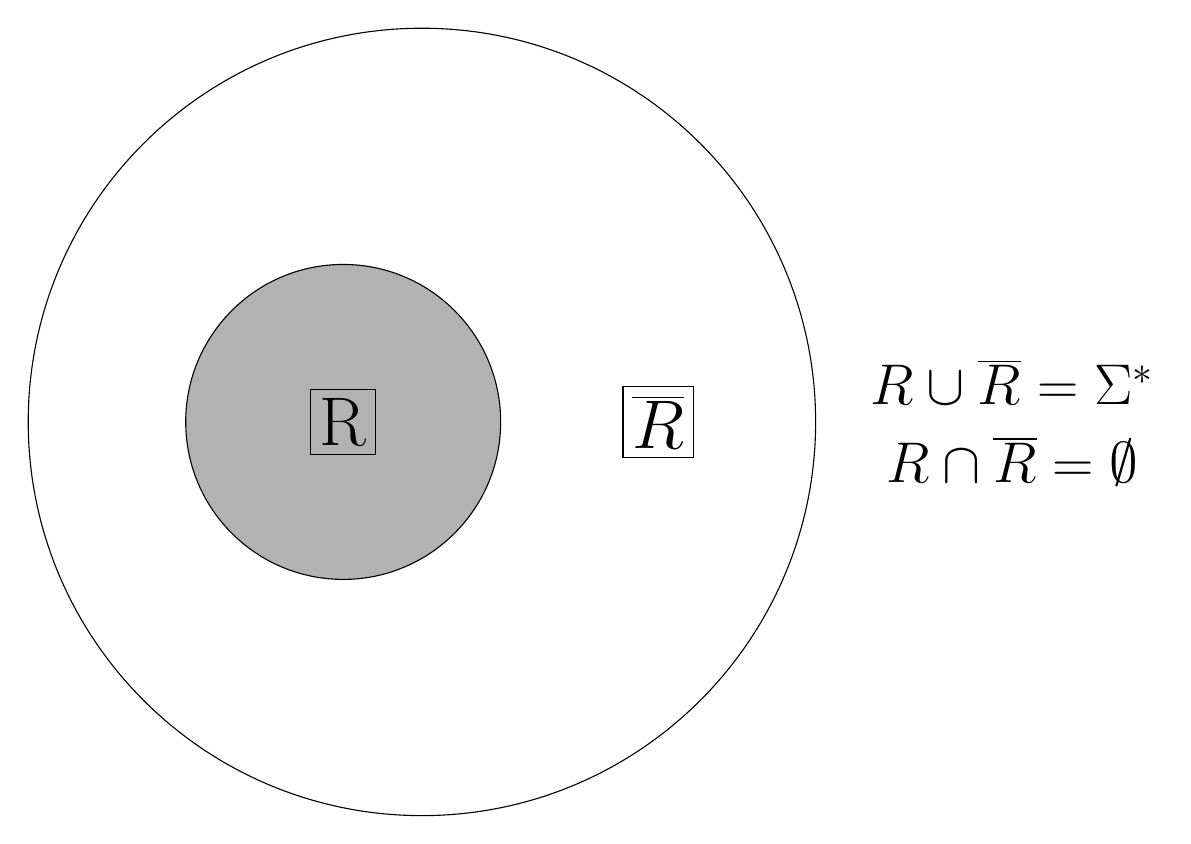
\begin{tikzpicture}
    \filldraw[fill=white, draw=black] (2,2) circle (5cm);
    \node [draw] at (5,2) {\Huge$\overline{R}$};
    \filldraw[fill=gray!60, draw=black] (1,2) circle (2cm);
    \node [draw] at (1,2) {\Huge R};
    \node at (9.5, 2.5) {\huge $R \cup \overline{R} = \Sigma^*$};
    \node at (9.5, 1.5) {\huge $R \cap \overline{R} = \emptyset$};
\end{tikzpicture}
    \caption{Regular language partition}
    \label{fig:tikz-reg-partition}
\end{figure}

\begin{figure}[!htb]
    \center
    \begin{tikzpicture}[scale = 0.5]
    \usetikzlibrary{calc}
    \node (a) [state] {\Huge$R \cup \overline{R} = \top = \Sigma^*$};
    \node (b1) [state, shift={($(a.south)+(3cm, -2.5cm)$)}] {\Huge $R$};
    \node (b2) [state, shift={($(a.south)+(-3cm, -2.5cm)$)}]{\Huge $\overline{R}$};
    \node (c) [state, shift= {($(a.south) + (0cm, -5.5cm)$)}] {\Huge $R \cap \overline{R} = \bot = \emptyset$};
    \draw (a) to (b1);
    \draw (a) to (b2);
    \draw (b1) to (c);
    \draw (b2) to (c);
\end{tikzpicture}
    \caption{Regular language partition as a lattice}
    \label{fig:tikz-reg-partition-lattice}
\end{figure}

\subsubsection{Abstract tuples}\label{subsubsec:abstract-tuples}

We define abstract tuples as the product cover-lattices of $\regexs$ and $\uints$ intertwined depending on the schema of the table.
The concretization function is defined as follows:


\begin{gather}
    \concrete^{v_1, v_2, \dots, v_n}_5 : \bigtimes_{i = 1}^{n}(\lookupcl(v_i)) \rightarrow \mathcal{P}\left(\bigtimes_{i = 1}^n \cc(\lookupcl(v_i)) \right)\\
    \begin{split}
        \concrete^{v_1, v_2, \dots, v_n}_5 & (\ab{e_1}, \ab{e_2}, \dots, \ab{e_n}) = \\
         &\concrete^{v_1}_6(\ab{e_1}) \times \concrete^{v_2}_6(\ab{e_2}) \times \dots \times \concrete^{v_n}_6(\ab{e_n})
    \end{split}
\end{gather}

\subsubsection{Abstract application variable values}
In the concrete semantics defined by~\cite{halder_abstract_2012}, application variables can be assigned to either singleton or lists of values.
As much as we can, we would like to distinguish between these two cases, therefore we introduce the set $\mathsf{Val} \; S$ of list and singleton values inductively defined as:


\begin{gather*}
    \inference{}{\bot \in \mathsf{Val} \; S} \quad
    \inference{s \in S}{\mathsf{Single} \; s \in \mathsf{Val} \; S}\\
    \inference{S' \subseteq S}{\mathsf{List} \; S' \in \mathsf{Val} \; S}
\end{gather*}


% todo this should be uncommented if we wan't to fix the galios connection.
% We define the partial order $\sqsubseteq$ of the lattice $(\mathsf{Val} \; A, \sqsubseteq, \sqcup, \sqcap)$ as follows:
% \begin{align}
%     \mathsf{List} \; S_1 &\sqsubseteq \mathsf{List} \; S_2 \iff \forall s_1 \in S_1, \; \exists s_2 \in S_2: \; s_1 \sqsubseteq s_2 \\
%     \mathsf{Single} \; s_1 &\sqsubseteq \mathsf{Single} \; s_2 \iff s_1 \sqsubseteq s_2 \\
%     \mathsf{Single} \; s &\sqsubseteq \mathsf{List} \; S \iff s \in S \\
%     \mathsf{List} \; S &\not\sqsubseteq \mathsf{Single} \; s
% \end{align}
% The join and meet $\sqcup$ and $\sqcap$ respectively is defined as follows here:
% \begin{align}
%     \mathsf{Single} \; s \sqcup \mathsf{List} \; S &= \mathsf{List} \; (S\sqcup\left\{ s \right\})\\
%     \mathsf{Single} \; s_1 \sqcup \mathsf{Single} \; s_2 &= \mathsf{Single} \; (s \sqcup s )\\
%     \mathsf{List} \; S_1 \sqcup \mathsf{List} \; S_2 &= \mathsf{List} \; (S_1 \sqcup S_2)\\
%     \mathsf{Single} \; s \sqcap \mathsf{List} \; S &= \mathsf{Single} \; s\\
%     \mathsf{List} \; S_1 \sqcap \mathsf{List} \; S_2 &= \mathsf{List} \; (S_1 \sqcap S_2)\\
%     \mathsf{Single} \; s_1 \sqcap \mathsf{Single} \; s_2 &= \mathsf{Single} \; (s_1 \sqcap s_2)\\
%     \mathsf{List} \ \emptyset \sqcap \mathsf{Single} \ s &= \ \perp
% \end{align}

It will be helpful to further overload the $\into$ operator for this type of values, therefore we define


\begin{align}
    \cdot \into C_X(S) &: \mathsf{Val} \; S \rightarrow \mathsf{Val} \; C_X(S) \\
    (\mathsf{Single} \; s) \into C_X(S) &= \mathsf{Single} \; (s \into C_X(S)) \\
    (\mathsf{List} \; S') \into C_X(S) &= \mathsf{List} \; (S' \into C_X\left(S\right))
\end{align}


And the following notation will also be helpful later:


\begin{align}
    s \in (\mathsf{Single} \; s') \iff s = s^\prime \\
    s \in (\mathsf{List} \; S) \ \iff \ s \in S.
\end{align}


We define the concretization of application variable values as:


\begin{gather}
    \concrete^v_{4a} : \mathsf{Val} \; \lookupcl(v) \rightarrow \mathcal{P}(\cc(\lookupcl(v))) \cup\mathcal{P}((\cc(\lookupcl(v)))^\star)\\
    \concrete^v_{4a}(\mathsf{Single} \; \ab{s}) = \concrete_6(\ab{s})\\
    \begin{split}
        \concrete^v_{4a}(\mathsf{List} \; \ab{S'}) = \bigcup_{n \in \mathbb{N}}\biggl\{&s_1, s_2, \dots, s_n \in (\cc(\lookupcl(v)))^n \\
        & \Big| \forall i \in \{1, 2, \dots, n\} : \exists \ab{s} \in \ab{S'} : s_i \in \concrete^v_6(\ab{s}) \biggr\}
    \end{split}
\end{gather}


For the purpose of proving soundness later we also overload $\gamma_{4a}$ as follows:


\begin{align}
    \concrete_{4a} &: \mathsf{Val} \; \regexs \rightarrow \mathcal{P}(\strs) \cup \mathcal{P}(\strs^\star)\\
    \concrete_{4a} &: \mathsf{Val} \; \uints \rightarrow \mathcal{P}(\nums) \cup \mathcal{P}(\nums^\star) \\
    \concrete_{4a} &: \mathsf{Val} \; \mathcal{P}(\bools) \rightarrow \mathcal{P}(\bools) \cup \mathcal{P}(\bools^\star)
\end{align}

With the same \emph{implementation} as above where $\bools = \{\true, \false, \mnull\}$.

\subsubsection{Abstract tables}\label{subsubsec:abstract_domain_of_tables}
We consider a concrete table $t$ as function from the domain of possible tuples in the table $\mathbf{TUP}$ to the codomain of natural numbers including $0$, $\mathbf{NAT}$:


\begin{equation}
    t : \mathbf{TUP} \rightarrow \mathbf{NAT}.\label{eq:equation-tup-nat}
\end{equation}


The function $t$ describes the number of a given tuple in a table.
We can then consider abstracting over a table $t$ by abstracting either the domain or codomain.
This gives rise to a taxonomy of abstract domains of tables shown in \autoref{tab:taxonomy_of_abstract_domain_of_tables}.
In \autoref{tab:taxonomy_of_abstract_domain_of_tables}, $\ab{\mathbf{TUP}}$ denotes an abstract domain of the set of possible tuples $\mathbf{TUP}$ (and analogous for $\mathbf{NAT}$).


\begin{table}
    \renewcommand{\arraystretch}{1.3}
    \caption{Taxonomy of Abstract Domains of Tables}
    \centering
    \begin{tabular}{c|l}
        \toprule
        Classification                  & Function                                \\ \midrule
        Bag of tuples                   & $\mathbf{TUP} \rightarrow \mathbf{NAT}$           \\
        Abstract bag of tuples          & $\mathbf{TUP} \rightarrow \ab{\mathbf{NAT}}$      \\
        Bag of abstract tuples          & $\ab{\mathbf{TUP}} \rightarrow \mathbf{NAT}$      \\
        Abstract bag of abstract tuples & $\ab{\mathbf{TUP}} \rightarrow \ab{\mathbf{NAT}}$ \\ \bottomrule
    \end{tabular}
    \label{tab:taxonomy_of_abstract_domain_of_tables}
\end{table}

One would classify the work in~\cite{halder_abstract_2012} as using bags of abstract tuples, and in this work, as previously mentioned, we will use abstract bags of abstract tuples.
In this work in particular we consider $\ab{\mathbf{TUP}}$ as given by the map $\lookupcl$, and $\ab{\mathbf{NAT}} = \{0, 0 \leq\}$.

We admit that this notion is a bit vague and informal, but displays the intuition.

Formalizing this, we consider $\ab{t} : \ab{\mathbf{TUP}} \rightarrow \ab{\mathbf{NAT}}$ to be represented as a single set $\ab{t'}$ instead, that is $\ab{t}({e}) = 0 \iff e \notin \ab{t'}$ and  $\ab{t}({e}) = (0 \leq) \iff e \in \ab{t'}$.

Further, as the form of an abstract table is given by the schema and the mapping $\lookupcl$ the final formalization for some table with name $v_d$ is then $\ab{t} \in \mathcal{P}\left(\bigtimes_{i = 1}^{n}\lookupcl(v_i)\right)$ for $attr(v_d) = (v_1, v_2, \dots, v_n)$, where $attr : \mathbb{V}_d \rightarrow \mathbb{V}_t^\star$ is given by the schema of the database.

As the concretization of an abstract table is a multi-set we need to define a map from the underlying set $S$ to the set of multi-sets over that underlying set before we can define the concretization itself, we denote that set $\mathcal{M}(S)$ and define it formally as:


\begin{equation}
    \mathcal{M}(S) = \{t | t : S \rightarrow \nums\}\label{eq:equation-nums}
\end{equation}


And thus we can define the concretization of a table, for $attr(v_d) = (v_1, v_2, \dots, v_n)$:


\begin{gather}
    \concrete^{v_d}_{4d} : \mathcal{P}\left(\bigtimes_{i = 1}^{n}\lookupcl(v_i)\right) \rightarrow \mathcal{M}\left(\bigtimes_{i = 1}^n \cc(\lookupcl(v_i))\right)\\
    \begin{split}
        \concrete^{v_d}_{4d}(\ab{t}) = \biggl\{ &t \in \mathcal{M}\Bigl(\bigtimes_{i = 1}^n \cc(\lookupcl(v_i))\Bigr) \Big|\\
        &\forall e \in t : \exists \ab{e} \in \ab{t} : e \in \concrete^{attr(v_d)}_5(\ab{e}) \biggr\}
    \end{split}
\end{gather}


\subsubsection{Abstract environments}
We define an abstract environment $\rho_{\ab{a}} \in \ab{\mathfrak{E}_a}$ mapping application variable names $v_a \in \mathbb{V}_a$ to abstract values, and $\rho_{\ab{d}} \in \ab{\mathfrak{E}_d}$ mapping table names $v_d \in \mathbb{V}_d$ to abstract tables.
Given the previously mentioned map $\lookupcl$ in \autoref{eq:lookupcl} we define:


\begin{align}
    \ab{\mathfrak{E}_a} &= \mathbb{V}_a \rightarrow \mathsf{Val} \; \left( \bigcup_{v_a \in \mathbb{V}_a} \lookupcl(v_a) \right) \\
    \ab{\mathfrak{E}_d} &= \mathbb{V}_d \rightarrow \bigcup_{v_d \in \mathbb{V}_d} \mathcal{P}\left(\bigtimes_{v_t \in attr(v_d)}\lookupcl(v_t)\right) \\
    \ab{\mathfrak{E}} &= \ab{\mathfrak{E}_a} \times \ab{\mathfrak{E}_d}
\end{align}


And the concrete counterparts:


\begin{align}
    \mathfrak{E}_a &= \mathbb{V}_a \rightarrow \nums^\star \cup \strs^\star \\
    \mathfrak{E}_d &= \mathbb{V}_d \rightarrow \bigcup_{v_d \in \mathbb{V}_d} \mathcal{M}\left(\bigtimes_{v_t \in attr(v_d)}\cc(\lookupcl(v_t))\right) \\
    \mathfrak{E} &= \mathfrak{E}_a \times \mathfrak{E}_d
\end{align}


And we define the concretization functions for environments as:


\begin{gather}
    \concrete_2 : \ab{\mathfrak{E}} \rightarrow \mathcal{P}(\mathfrak{E})\\
    \concrete_2(\rho_{\ab{d}}, \rho_{\ab{a}}) = \concrete_{3d}(\rho_{\ab{d}}) \times \concrete_{3a}(\rho_{\ab{a}})
\end{gather}


\begin{gather}
    \concrete_{3d} : \ab{\mathfrak{E}_d} \rightarrow \mathcal{P}(\mathfrak{E}_d)\\
    \concrete_{3d}(\rho_{\ab{d}}) = \biggl\{ \rho_{a} \in \mathfrak{E}_d \Big| \forall v_d \in \mathbb{V}_d : \rho_d(v_d) \in \concrete^{v_d}_{4d}(\rho_{\ab{d}}(v_d)) \biggr\}
\end{gather}


\begin{gather}
    \concrete_{3a} : \ab{\mathfrak{E}_a} \rightarrow \mathcal{P}(\mathfrak{E}_a)\\
    \concrete_{3a}(\rho_{\ab{a}}) = \biggl\{ \rho_{a} \in \mathfrak{E}_a \Big| \forall v_a \in \mathbb{V}_a : \rho_a(v_a) \in \concrete^{v_a}_{4a}(\rho_{\ab{a}}(v_a)) \biggr\}
\end{gather}


And in the same vain we define a concretization function for sets of environments as:


\begin{gather}
    \concrete_1 : \mathcal{P}(\ab{\mathfrak{E}}) \rightarrow \mathcal{P}(\mathfrak{E})\\
    \begin{split}
        \concrete_1(\ab{P}) = \biggl\{ &(\rho_{d}, \rho_{a}) \in \mathfrak{E} \\
        &\Big| \exists (\rho_{\ab{d}}, \rho_{\ab{a}}) \in \ab{P} : (\rho_{d}, \rho_{a}) \in \concrete_2(\rho_{\ab{d}}, \rho_{\ab{a}})\biggr\}
    \end{split}
\end{gather}

